%Réplique de la mission InSIGHT

L'étude proposée porte sur la réplique terrestre\footnote{Utilisée sur Terre pour validation des différents sous-systèmes.} du système InSIGHT (Interior exploration using
Seismic Investigations, Geodesy and Heat Transport), projet du CNES (Centre National d’Études
Spatiales) qui a pour but de déployer une station d'étude de la structure interne de la planète Mars.
La station de mesures doit effectuer une campagne de mesures de l'activité sismique afin d'établir des
informations sur l'épaisseur de la croûte martienne, de ses manteaux et des zones de subduction, voire
des impacts des météorites.
Le support technologique de la mission est un atterrisseur similaire à celui de la mission Phoenix qui
a été utilisé avec succès en 2007 pour étudier le sol glacé près du pôle nord de Mars.

\begin{figure}[!h]
\centering
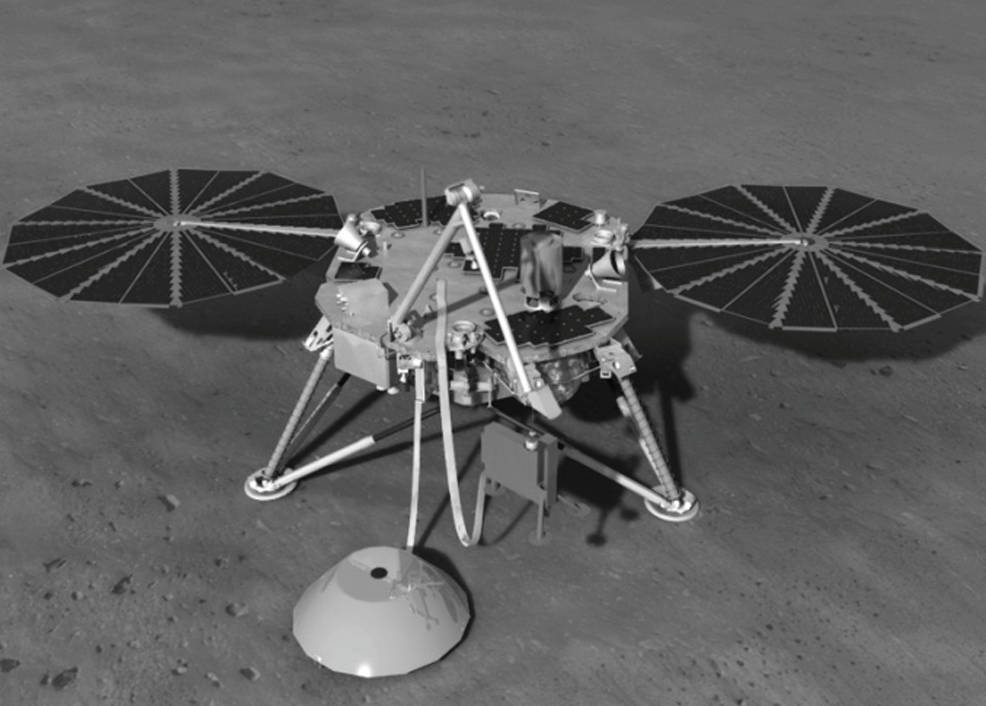
\includegraphics[width=.7\linewidth]{ccinp_mp2019_fig_01.png}
\caption{Atterrisseur du projet InSIGHT \label{ccinp_mp2019_fig_01}}
\end{figure}



L'atterrisseur InSIGHT (figure \ref{ccinp_mp2019_fig_01}) emportera quatre sous-systèmes d’instrumentation à la surface de
Mars afin d’analyser en détail pour la première fois les "statistiques vitales" de la planète :
\begin{itemize}
\item son pouls, activité interne, mesuré par l'instrument SEIS ;
\item sa température mesurée par l'instrument HP³ ;
\item ses réflexes mesurés par l'instrument RISE.
\end{itemize}
Ensemble, les données fourniront des indices essentiels sur l'évolution, non seulement de la planète
Mars, mais aussi de toutes les planètes telluriques.
Sous-systèmes d’instrumentation de l’atterrisseur
\begin{itemize}
\item SEIS : sismomètre qui fera des mesures précises des tremblements et autres activités internes
de Mars pour mieux comprendre l'histoire et la structure de la planète ;
\item HP³ : cet instrument va s’enfoncer, à cinq mètres de profondeur sous la surface de Mars, pour
connaître la quantité de chaleur venant de l'intérieur de Mars et pour révéler l'histoire
thermique de la planète ;
\item RISE : il s’agit d’une expérience qui mesurera avec précision le décalage Doppler et le
parcours des communications radio entre l'atterrisseur InSIGHT et la Terre pour déterminer
la distribution des structures internes de la planète rouge ;
\item Camera : montée sur le bras de l'atterrisseur, elle servira à prendre des images en noir et blanc
des instruments sur le corps de l'atterrisseur ainsi qu'une vue en 3D pour aider les ingénieurs
et les scientifiques à guider le déploiement des instruments au sol. 
\end{itemize}


 Seul le sous-système SEIS (figure \ref{ccinp_mp2019_fig_02}) sera l’objet de l’étude proposée.Il est basé sur un instrument hybride composé:
\begin{itemize}
\item d'un système de déploiement (DPL);
\item d'unesphère comportant trois capteurs sismiques àtrès largesbandeset leurs capteurs de 
température.La sphère dispose d’un système de référencement de ses pieds (figure \ref{ccinp_mp2019_fig_03}). Sa masse est d'environ \SI{3}{kg} et sa consommation électrique varie autour de \SI{1}{W}.
 \item d'une boîte électronique d'acquisition dont la structure est donnée par le diagramme de 
définition des blocs de la figure \ref{ccinp_mp2019_fig_04}.
\end{itemize}


\begin{minipage}[c]{.47\linewidth}
\begin{center}
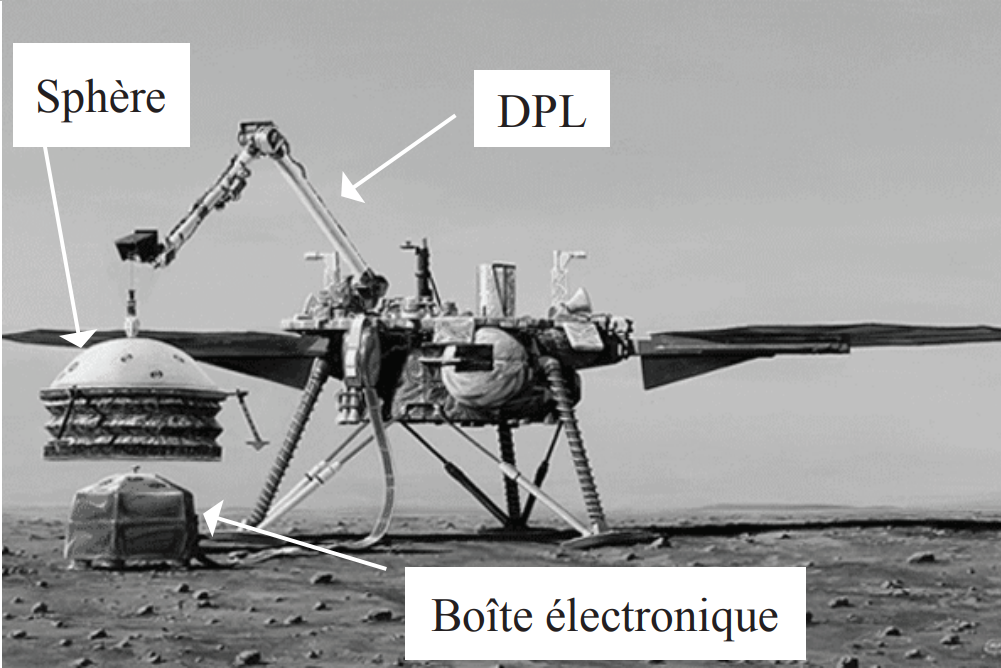
\includegraphics[width=.9\linewidth]{ccinp_mp2019_fig_02.png}
\captionof{figure}{Ensemble SEIS en phase de déploiement \label{ccinp_mp2019_fig_02}}
\end{center}
\end{minipage} \hfill
\begin{minipage}[c]{.47\linewidth}
\begin{center}
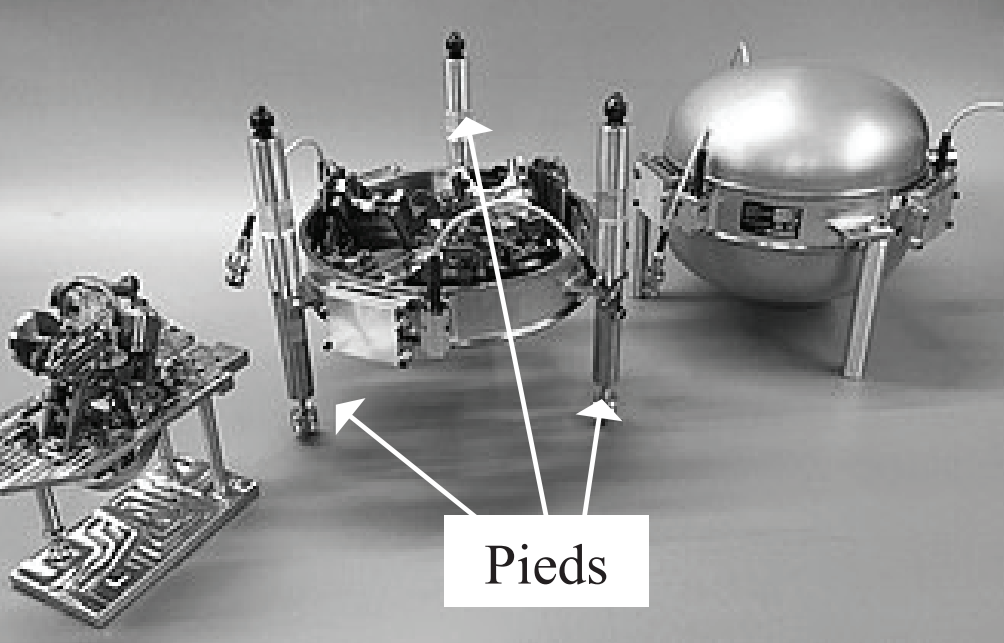
\includegraphics[width=.9\linewidth]{ccinp_mp2019_fig_03.png}
\captionof{figure}{Sphère SEIS \label{ccinp_mp2019_fig_03}}
\end{center}
\end{minipage}

\begin{figure}[!h]
\centering
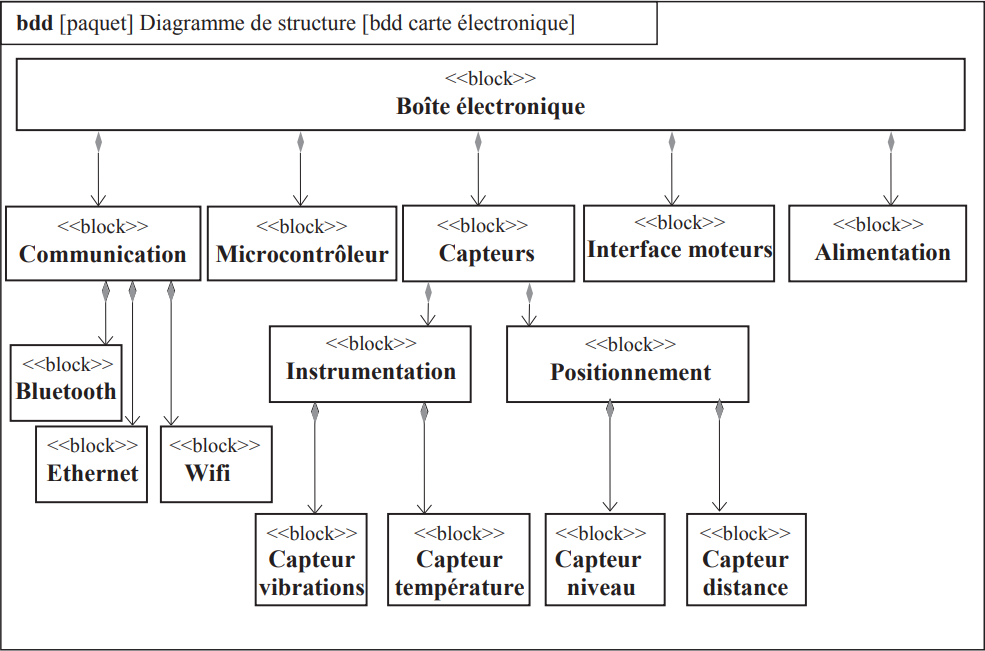
\includegraphics[width=\linewidth]{ccinp_mp2019_fig_04.png}
\caption{Diagramme de définition des blocs \label{ccinp_mp2019_fig_04}}
\end{figure}

La figure \ref{ccinp_mp2019_fig_05} présente le diagramme des cas d'utilisation du système de positionnement DPL et du module SEIS et la figure \ref{ccinp_mp2019_fig_06} le diagramme partiel des exigences concernant le système de déploiement DPL et le module SEIS.



\begin{figure}[!h]
\centering
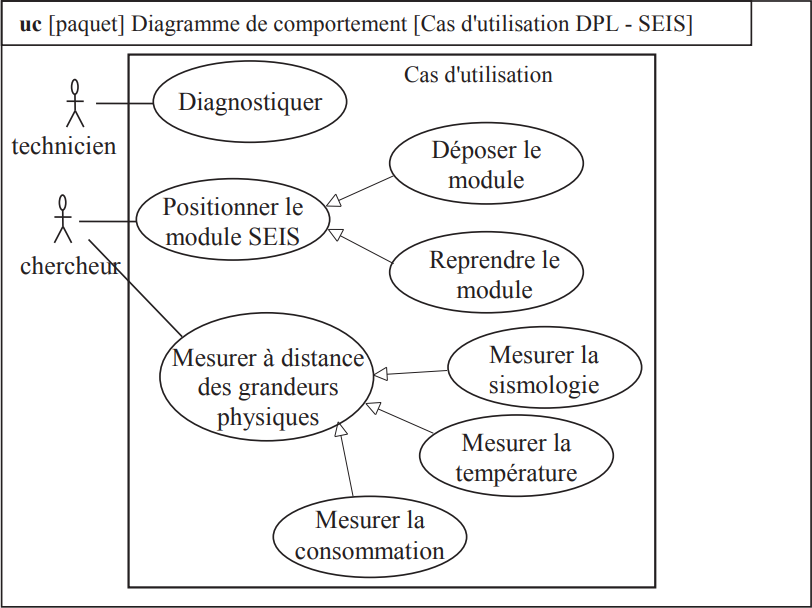
\includegraphics[width=.7\linewidth]{ccinp_mp2019_fig_05.png}
\caption{Diagramme des cas d'utilisation\label{ccinp_mp2019_fig_05}}
\end{figure}

\begin{figure}[!h]
\centering
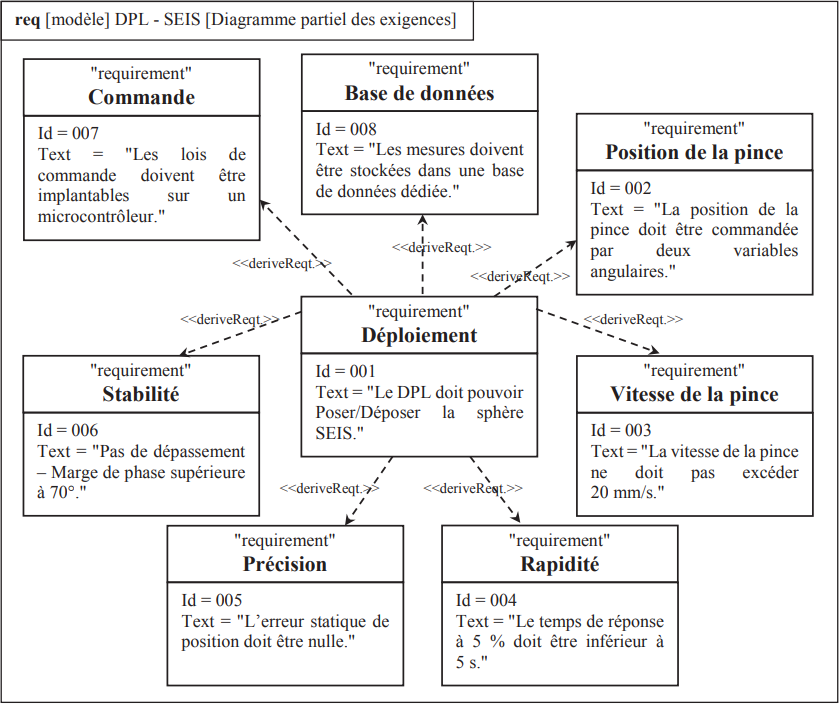
\includegraphics[width=.9\linewidth]{ccinp_mp2019_fig_06.png}
\caption{Diagramme partiel des exigences \label{ccinp_mp2019_fig_06}}
\end{figure}

 La figure \ref{ccinp_mp2019_fig_07} représente la structure du système de déploiement DPL. 


\begin{figure}[!h]
\centering
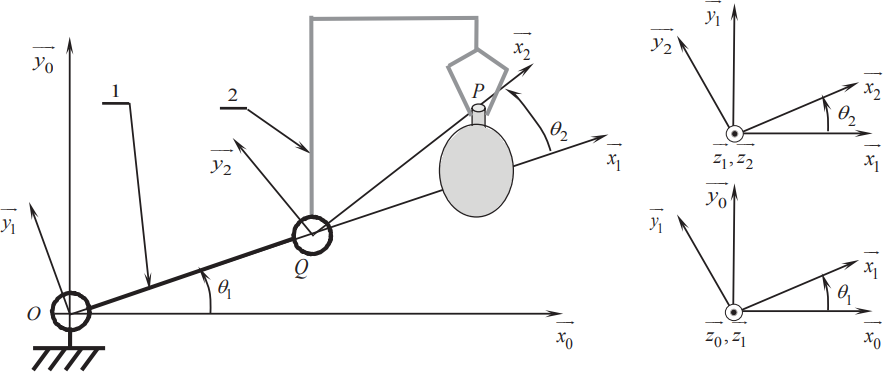
\includegraphics[width=\linewidth]{ccinp_mp2019_fig_07.png}
\caption{Schématisation cinématique du bras de déploiement \label{ccinp_mp2019_fig_07}}
\end{figure}


\paragraph*{Bâti 0}
Le bâti 0 est doté du repère $\rep{0} \repere{O}{x_0}{y_0}{z_0}$.

\paragraph*{Bras 1}

Le bras 1 est doté du repère $\rep{1} \repere{O}{x_1}{y_1}{z_1}$. Le mouvement de 1 par rapport à 0 est une rotation d'axe $\axe{O}{z_0}$  et d'angle $\theta_1 = \angl{x_0}{x_1}= \angl{y_0}{y_1}$. Le centre d'inertie $G_1$ est paramétré par $\vect{OG_1} = \dfrac{L}{2} \vx{1}$. De plus $\vect{OQ} = L\vx{1}$. Enfin, $m_1 = \SI{352}{g}$ et $L=\SI{0,5}{m}$.

La figure \ref{ccinp_mp2019_fig_08} présente le modèle volumique du bras 1. Les plans $\left(G_1, \vx{1},\vy{1} \right)$  et $\left(G_1,\vy{1},\vz{1}\right)$ sont des plans de symétrie matérielle du bras 1.

\begin{figure}[!h]
\centering
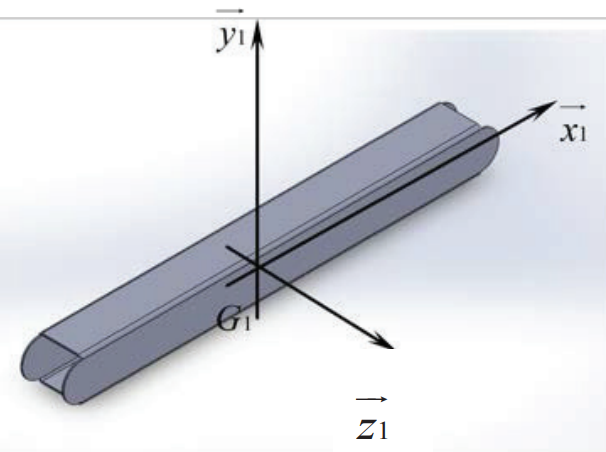
\includegraphics[width=.45\linewidth]{ccinp_mp2019_fig_08.png}
\caption{Bras 1\label{ccinp_mp2019_fig_08}}
\end{figure}

Le mouvement de 1 par rapport à 0 est commandé par un actionneur $\indice{M}{01}$, constitué d’un moteur pas à pas et d’un réducteur de vitesse à couronne dentée flexible de rapport de transmission $\lambda = 82$, d’encombrement et de masse très faibles en regard des autres solides, logés à l’intérieur de la liaison (0/1).


\paragraph*{Avant-bras 2}
L'avant-bras 2 est doté du repère $\rep{2} \repere{Q}{x_2}{y_2}{z_2}$. Le mouvement de 2 par rapport à 0 est une rotation d'axe $\axe{Q}{z_1}$  et d'angle $\theta_2 = \angl{x_1}{x_2}= \angl{y_1}{y_2}$. Le centre d'inertie $G_2$ est paramétré par $\vect{OG_2} = \dfrac{L}{2} \vx{2}$. De plus $\vect{QP} = L\vx{2}$. Enfin, $m_2 = \SI{352}{g}$ et $L=\SI{0,5}{m}$.

L’extrémité en $P$ est équipée d’une pince de masse négligeable qui saisit la sphère SEIS. On note $\indice{K}{O2}$ le moment d'inertie de l'avant-bras 2 par rapport à l’axe $\axe{O}{z_0}$ dans la position la plus défavorable.  Le mouvement de 2 par rapport à 1 est commandé par un actionneur $\indice{M}{12}$, constitué d’un moteur pas à pas et d’un réducteur de vitesse à couronne dentée flexible de rapport de transmission $\lambda = 82$, d’encombrement et de masse très faibles en regard des autres solides, logés à l’intérieur de la liaison (1/2).


\paragraph*{Sphère du SEIS : S}
On considère que l’amplitude du mouvement (S/2) est très faible. La position (S/0) repérée par : $\vect{OP}= X_P(t) \vx{0} + Y_P(t) \vy{0} $. La masse $m_s = \SI{1,2}{kg}$ est considérée comme ponctuelle en son centre d’inertie $G_S$  par rapport aux autres mouvements. $G_S$  est tel que $\vect{PG_S} = -R \vy{0}$ ($R$ est une constante positive).

On note $\indice{K}{OS}$ le moment d'inertie de la sphère $S$ par rapport à l’axe $\axe{O}{z_0}$  dans la position $\theta_1 =\theta_2 = 0$.

